\documentclass[runningheads,a4paper,11pt]{report}

\usepackage{algorithmic}
\usepackage{algorithm} 
\usepackage{array}
\usepackage{amsmath}
\usepackage{amsfonts}
\usepackage{amssymb}
\usepackage{amsthm}
\usepackage{caption}
\usepackage{comment} 
\usepackage{epsfig} 
\usepackage{fancyhdr}
\usepackage[T1]{fontenc}
\usepackage{geometry} 
\usepackage{graphicx}
\usepackage[colorlinks]{hyperref} 
\usepackage[latin1]{inputenc}
\usepackage{multicol}
\usepackage{multirow} 
\usepackage{rotating}
\usepackage{setspace}
\usepackage{subfigure}
\usepackage{url}
\usepackage{float}
\usepackage{verbatim}
\usepackage{xcolor}
\usepackage{float} % Include this in the preamble


\geometry{a4paper,top=2cm,left=2.5cm,right=2cm,bottom=2cm}

\renewcommand{\headrulewidth}{2pt}
\renewcommand{\footrulewidth}{2pt}
\renewcommand{\headrule}{\hbox to\headwidth{%
  \color{lime}\leaders\hrule height \headrulewidth\hfill}}
\renewcommand{\footrule}{\hbox to\headwidth{%
  \color{lime}\leaders\hrule height \footrulewidth\hfill}}

\hypersetup{
pdftitle={artTitle},
pdfauthor={name},
pdfkeywords={pdf, latex, tex, ps2pdf, dvipdfm, pdflatex},
bookmarksnumbered,
pdfstartview={FitH},
urlcolor=cyan,
colorlinks=true,
linkcolor=lightblue,
citecolor=cyan,
}
% \pagestyle{plain}

\setcounter{secnumdepth}{3}
\setcounter{tocdepth}{3}

\linespread{1}

% \pagestyle{myheadings}

\makeindex

\begin{document}

\begin{titlepage}
\sloppy

\begin{center}
BABE\c S BOLYAI UNIVERSITY, CLUJ NAPOCA, ROM\^ ANIA

FACULTY OF MATHEMATICS AND COMPUTER SCIENCE

\vspace{5cm}

\Huge \textbf{Early Discovery of Anxiety/Depression in Teenagers Using Digital Tools}

\vspace{1cm}

\normalsize -- MIRPR report --

\end{center}


\vspace{5cm}

\begin{flushright}
\Large{\textbf{Toth Alexandra-Melania \\ Vl\u{a}d\u{a}u Andra-Ioana \\ Mihalcea Ioan-Alexandu}}\\
\textbf {Emails: }
alexandra.melania.toth@stud.ubbcluj.ro, 
andra.vladau@stud.ubbcluj.ro, 
ioan.mihalcea@stud.ubbcluj.ro\\
\textbf{ Specialisation:} Computer Science Romanian
\end{flushright}

\vspace{2cm}


\begin{center}
2024-2025
\end{center}

\end{titlepage}

\pagenumbering{gobble}

\tableofcontents

\newpage

\listoffigures

\newpage



\newpage

\pagenumbering{arabic}


\chapter{Introduction}
\label{chapter:introduction}


\section{Objective:}
\label{section:objective}
Anxiety/Depression for teenagers - To enhance mental health support for teenagers by developing digital tools that can proactively identify signs of anxiety and depression. These tools aim to engage adolescents in their digital environments, whether through chatbots, social media, video games, or other innovative platforms, to provide early intervention and emotional support.


\section{Main Idea:}
\label{section:idea}
The Early Discovery of Anxiety/Depression in Teenagers solution uses digital platforms to identify and monitor mental health challenges among adolescents. The system combines multiple approaches, including AI-powered chatbots capable of conversational analysis, sentiment evaluation through social media interactions, and mental health assessments embedded in video game experiences. By engaging teenagers where they spend most of their time, be it online or in games, the system aims to provide real-time insights and early warnings of anxiety or depression. This integrated solution offers a holistic approach, blending digital engagement with predictive analytics and personalized intervention strategies.

\section{Motivation:}
\label{section:motivation}
Teen anxiety and depression are pressing issues, often going unnoticed due to social stigma, lack of awareness, or teens' reluctance to seek help. Traditional detection methods are limited in reach and timing, missing critical opportunities for early intervention. By embedding intelligent algorithms in digital spaces where teens naturally engage, like social media, chat apps, and video games, we can monitor signs of mental distress in real time.

AI-powered tools, especially those using natural language processing and machine learning, can analyze behavioural patterns, detect early signs of anxiety or depression, and respond immediately, offering instant, personalized support. These algorithms not only provide proactive intervention, but also reduce barriers to help seek by creating a safe, accessible way for adolescents to explore mental health support in familiar digital environments. This intelligent approach can help prevent more serious issues, offering timely and compassionate care to teens who need it most.


\chapter{The Scientific Problem Addressed}
\label{chapter:scientific}

The prevalence of anxiety and depression among teenagers has reached alarming levels in recent years, with studies indicating a sharp increase in mental health issues within this demographic. According to the World Health Organization (WHO), nearly 10 - 20\% of adolescents worldwide experience mental health conditions, with many cases undiagnosed and untreated. These issues, if unaddressed, can lead to long-term psychological, academic, and social consequences.

A significant challenge in addressing teenage mental health lies in early detection of symptoms. Adolescents often hesitate to seek help due to stigma, lack of awareness, or limited access to traditional healthcare services. Additionally, current diagnostic methods rely heavily on self-reporting or clinical observations, which may not capture the nuanced and early signs of anxiety and depression.

In the digital age, teenagers increasingly interact with technology, spending substantial amounts of time on social media platforms, messaging apps, and video games. These environments often capture behavioral patterns and emotional cues that can serve as indicators of mental health challenges. However, traditional mental health interventions have largely overlooked the potential of these digital spaces to provide proactive and non-intrusive support.

The scientific problem addressed by this project centers on bridging this gap by leveraging advanced digital tools to identify, monitor, and provide early interventions for anxiety and depression. Specifically, the project seeks to answer the following key questions:
\begin{itemize}
    \item How can artificial intelligence and sentiment analysis be utilized to identify early signs of anxiety and depression in teenagers through their digital interactions?
    \item What methods can effectively integrate mental health assessments into engaging and non-invasive digital environments such as video games and chatbots?
    \item How can predictive analytics be used to ensure timely and personalized interventions for at-risk adolescents?
\end{itemize}

By addressing these questions, this project aims to create an innovative, evidence-based approach to teenage mental health care. It leverages the ubiquity of digital platforms to provide scalable, accessible, and proactive solutions to a growing global health challenge.


\chapter{Existing Problem-Solving Methods (Related Work)}
\label{chapter:existing-problem}
This chapter provides an in-depth exploration of the algorithms applied to the problem of mental health classification, the methodologies for learning and optimization, and the metrics employed to evaluate the quality of solutions. The focus is on understanding the mechanisms, utility, limitations, and examples of the algorithms, as well as how their outputs are measured to ensure effective decision-making.

\section{Algorithms Used}
\label{section:algorithms_used}

\subsection{Support Vector Machine (SVM)}
\label{subsection:svm}

\subsubsection{How it works}
\label{subsubsection:svm_how_it_works}

Support Vector Machine (SVM) is a supervised learning algorithm designed for binary and multiclass classification tasks. Its primary objective is to find the best possible hyperplane to separate data points belonging to different classes. For linearly separable data, SVM identifies the hyperplane that maximizes the margin between classes. When data is non-linear, SVM employs kernel functions such as Radial Basis Function (RBF) or polynomial kernels to map the data into a higher-dimensional space where separation becomes feasible.

\subsubsection{Why it is useful}
\label{subsubsection:svm_why_useful}

SVM is particularly effective in smaller datasets with distinct boundaries between classes, making it well-suited for the structured survey responses used in this study. It performs well in high-dimensional spaces and offers a robust mathematical foundation for classification. Additionally, its use of kernel functions allows for flexibility in handling non-linear data.

\subsubsection{Limitations}
\label{subsubsection:svm_limitations}

Despite its strengths, SVM struggles with large datasets due to computational intensity, as its training time scales quadratically with the dataset size. Additionally, it is sensitive to outliers, which can significantly influence the decision boundary. Selecting the correct kernel and hyperparameters requires extensive experimentation, which can be time-consuming.

\subsubsection{Examples}
\label{subsubsection:svm_examples}

In the context of mental health classification, SVM was used to analyze text features extracted from survey data. For example, responses like \textit{``I feel constantly worried''} may be classified as \textit{Anxiety}, while \textit{``I feel hopeless''} may be categorized as \textit{Depression}, using patterns in word frequency and semantics.

\subsection{Linear Regression}
\label{subsection:linear_regression}

\subsubsection{How it works}
\label{subsubsection:linear_regression_how_it_works}

Linear regression is a simple, interpretable model that assumes a linear relationship between input features and the target variable. In this study, it is used for multiclass classification by representing each sentence as a numerical vector of features (e.g., word frequencies or sentiment scores). The algorithm calculates weights for these features to predict the probability of a sentence belonging to a specific class.

\subsubsection{Why it is useful}
\label{subsubsection:linear_regression_why_useful}

Linear regression offers simplicity and interpretability, making it a suitable baseline algorithm for understanding the data and relationships between features. It is computationally inexpensive, allowing for rapid prototyping and testing.

\subsubsection{Limitations}
\label{subsubsection:linear_regression_limitations}

Its reliance on linear assumptions limits its applicability to more complex datasets, where interactions between features or non-linear patterns are critical. Linear regression may also fail to perform well in cases of high feature dimensionality or multicollinearity.

\subsubsection{Examples}
\label{subsubsection:linear_regression_examples}

For example, the model may classify sentences like \textit{``I am happy''} or \textit{``I cannot focus''} based on sentiment scores calculated from word frequencies. If the sentiment score is positive, the model might classify the sentence as \textit{Normal}, while negative scores may correspond to \textit{Depression} or \textit{Anxiety}.

\subsection{Decision Tree}
\label{subsection:decision_tree}

\subsubsection{How it works}
\label{subsubsection:decision_tree_how_it_works}

Decision trees are a supervised learning algorithm used for classification and regression tasks. They function by splitting the dataset into subsets based on feature values, creating a tree-like structure of decisions. In this study, decision trees work alongside sentence embeddings generated by the \textit{all-MiniLM-L6-v2} transformer model. These embeddings provide a rich, semantic representation of the input data, which the decision tree uses to make splits at each node.

\subsubsection{Why it is useful}
\label{subsubsection:decision_tree_why_useful}

Decision trees are easy to interpret and can handle both numerical and categorical data. When paired with transformer-generated embeddings, they can effectively model complex relationships within the data. Their non-parametric nature allows them to capture non-linear patterns, making them versatile for text-based classification tasks.

\subsubsection{Limitations}
\label{subsubsection:decision_tree_limitations}

Decision trees are prone to overfitting, especially when the tree depth is not constrained. They can also be sensitive to noise in the data, which might lead to less robust predictions. Additionally, they may struggle with high-dimensional data unless used with dimensionality reduction techniques or well-structured embeddings like those from transformers.

\subsubsection{Examples}
\label{subsubsection:decision_tree_examples}

For instance, responses encoded using \textit{all-MiniLM-L6-v2}, such as \textit{``I feel constantly tired and unmotivated,''} are processed by the decision tree to predict classes like \textit{Depression} or \textit{Fatigue}. The embeddings enable the decision tree to consider the semantic context of the response.

\subsection{Neural Networks with Transformers (Sentence Transformers)}
\label{subsection:transformers}

\subsubsection{How it works}
\label{subsubsection:transformers_how_it_works}

Transformer models such as \textit{all-MiniLM-L6-v2} are based on the attention mechanism, enabling them to focus on important aspects of input data while processing sequences of text. These models use a neural network architecture that converts input sentences into numerical embeddings. These embeddings capture the semantic meaning of each sentence and its context within the overall dataset. By leveraging the power of pre-trained embeddings, the algorithm can quickly generalize to new tasks with minimal fine-tuning.

\subsubsection{Why it is useful}
\label{subsubsection:transformers_why_useful}

Transformers are particularly well-suited for analyzing natural language data because they excel at capturing the subtleties of sentence meaning and relationships. Their ability to handle unstructured data makes them indispensable for tasks involving text classification or understanding complex linguistic patterns. They also allow for transfer learning, which reduces the computational cost of training from scratch.

\subsubsection{Limitations}
\label{subsubsection:transformers_limitations}

The primary limitation of transformers lies in their computational requirements, both in terms of memory and processing power. This makes them slower to train and deploy compared to traditional algorithms. Additionally, they can overfit on smaller datasets, necessitating careful fine-tuning or the use of regularization techniques.

\subsubsection{Examples}
\label{subsubsection:transformers_examples}

For instance, a response like \textit{``I feel overwhelmed by my responsibilities''} is encoded into a high-dimensional vector representing its semantic meaning. The transformer model identifies the closest match based on training data, categorizing this response as \textit{Anxiety}.

\subsection{Random Forest Classifier}
\label{subsection:random_forest}

\subsubsection{How it works}
\label{subsubsection:random_forest_how_it_works}

Random Forest is an ensemble learning algorithm that builds multiple decision trees during training and merges their outputs to improve classification accuracy. In this study, the algorithm works with text data represented as TF-IDF vectors. TF-IDF (Term Frequency-Inverse Document Frequency) captures the importance of words in the dataset by quantifying their frequency and uniqueness. The random forest aggregates the predictions from individual trees to classify text responses.

\subsubsection{Why it is useful}
\label{subsubsection:random_forest_why_useful}

Random Forest is robust to overfitting and performs well on a wide range of classification problems. Its ability to handle high-dimensional data makes it suitable for text classification tasks. Additionally, by using TF-IDF features, the algorithm can focus on the most informative terms in the text data.

\subsubsection{Limitations}
\label{subsubsection:random_forest_limitations}

The algorithm requires more computational resources compared to single decision trees. It can also become less interpretable as the number of trees increases. Additionally, the performance of Random Forest depends on the quality of the features; poorly chosen features may lead to suboptimal results.

\subsubsection{Examples}
\label{subsubsection:random_forest_examples}

For example, TF-IDF vectors representing responses like \textit{``I am unable to concentrate and feel restless''} are fed into the Random Forest classifier. By analyzing the importance of terms like \textit{``concentrate''} and \textit{``restless,''} the algorithm predicts classes such as \textit{Anxiety} or \textit{ADHD}.

\section{Learning/Optimization Process}
\label{section:learning_optimization}

The learning process involves the training and fine-tuning of the algorithms discussed above to maximize their performance on the classification task. Training data was divided into labeled classes, allowing supervised learning techniques to map input features to output classes. The optimization process involved selecting appropriate hyperparameters, such as:
\begin{itemize}
    \item The choice of kernel for SVM (e.g., RBF kernel for non-linear data).
    \item Fine-tuning pre-trained transformer models for sentence classification.
    \item Adjusting regularization parameters for linear regression to avoid overfitting.
    \item Limiting the depth of decision trees to prevent overfitting.
    \item Optimizing the number of trees in the Random Forest to balance accuracy and computational cost.
\end{itemize}

The performance of each model was validated using techniques like cross-validation to ensure generalization to unseen data.

\section{Metrics for Assessing Solution Quality}
\label{section:metrics_quality}

The quality of each algorithm's predictions was assessed using the following metrics:
\begin{itemize}
    \item \textbf{Accuracy} -- The proportion of correct predictions made by the model across all classes.
    \item \textbf{Precision, Recall, and F1-Score} -- These metrics provide a detailed view of performance for imbalanced datasets:
    \begin{itemize}
        \item \textbf{Precision} measures the accuracy of positive predictions.
        \item \textbf{Recall} evaluates the algorithm's ability to capture all relevant instances.
    \end{itemize}
    \item \textbf{Confusion Matrix} -- A visualization of true vs. predicted labels for each class, highlighting errors and their distribution.
    
\end{itemize}

These metrics collectively ensured that the solutions were robust, accurate, and suitable for real-world application.



\chapter{Experimental results obtained}
\label{chapter:experimental-results}

\section{Description of the Datasets}
\label{section:description}
This study leverages five publicly available datasets sourced from Kaggle to develop and evaluate the proposed digital tools for the early detection of anxiety and depression in teenagers. These datasets include the \textbf{Depression Reddit Dataset (Cleaned)} \cite{depression_reddit_cleaned}, the \textbf{Emotion Recognition Dataset} \cite{emotion_dataset}, the \textbf{Emotions Dataset} \cite{emotions}, the \textbf{Reddit Mental Health Dataset} \cite{reddit_dataset} and the \textbf{Students Anxiety and Depression Dataset} \cite{students_anxiety_depression}. 

\subsection{The Datasets}
\label{section:datasets}

\subsubsection{Reddit Mental Health Dataset}
\label{section:reddit}
The \textbf{Reddit Mental Health Dataset} contains posts from Reddit users, labeled based on various mental health conditions. For this project, we focused on two relevant categories: \textit{Anxiety} and \textit{Depression}. The dataset originally includes the following categories:
\begin{itemize}
    \item 0: Stress
    \item 1: Depression
    \item 2: Bipolar Disorder
    \item 3: Personality Disorder
    \item 4: Anxiety
\end{itemize}
For our analysis, only posts labeled as \textit{Depression} and \textit{Anxiety} were retained. The \textit{title} column was removed, and the data was concatenated with the \textbf{Emotion Recognition Dataset}. To ensure data consistency, null values were removed, and the dataset was balanced to prevent bias towards the larger class.

\subsubsection{Emotion Recognition Dataset}
\label{section:emotion}
The \textbf{Emotion Recognition Dataset} includes text samples labeled with six emotion categories:
\begin{itemize}
    \item 0: Anger
    \item 1: Fear
    \item 2: Joy
    \item 3: Love
    \item 4: Sadness
    \item 5: Surprise
\end{itemize}
The labels were transformed into three broader categories to align with our focus on mental health:
\begin{itemize}
    \item \textbf{Anxiety:} Includes posts labeled as \textit{Fear} and \textit{Surprise}.
    \item \textbf{Depression:} Includes posts labeled as \textit{Sadness} and \textit{Anger}.
    \item \textbf{Normal:} Includes posts labeled as \textit{Joy} and \textit{Love}.
\end{itemize}

The resulting dataset combines information from both sources, providing a diverse set of features for model training and evaluation. Oversampling was applied to the \textit{Normal} class to balance its representation with \textit{Anxiety} and \textit{Depression}.

\subsection{Quantitative Analysis of the Datasets}
\label{section:analysis}

\textbf{Small Dataset:} For initial experiments and prototyping, we created a smaller subset by selecting the first 500 rows from each category (\textit{Anxiety} and \textit{Depression}), resulting in a balanced dataset of 1,000 rows.

\textbf{Large Dataset:} The larger dataset used for final model training and testing contains:
\begin{itemize}
    \item \textbf{Anxiety:} 20,290 rows
    \item \textbf{Depression:} 21,796 rows
\end{itemize}
This dataset provides a robust foundation for training predictive models and evaluating their performance.

\subsection{Related Work and Usage of Datasets}
\label{section:usage}
Both datasets have been used in prior research to analyze mental health and emotional patterns through text. For instance:
\begin{itemize}
    \item The \textbf{Reddit Mental Health Dataset} has been utilized to study language patterns associated with mental health conditions and develop classification models for mental health prediction. Studies have achieved notable accuracy in identifying conditions like anxiety and depression using natural language processing (NLP) techniques.
    \item The \textbf{Emotion Recognition Dataset} has been widely used for emotion classification tasks, leveraging machine learning models to distinguish between different emotional states.
\end{itemize}

In this project, we extend these works by combining both datasets, re-labeling their categories to focus specifically on anxiety, depression, and normal states, and balancing the data to enhance model performance. By addressing class imbalances and tailoring the datasets to the problem, we aim to improve the detection of mental health conditions in digital interactions.

\subsection{Preprocessing and Data Transformation}
\label{section:preprocessing}
\begin{itemize}
    \item Extracted relevant labels and mapped them to \textit{Depression}, \textit{Anxiety}, and \textit{Normal}.
    \item Removed unnecessary columns such as \textit{title} from the Reddit dataset.
    \item Checked and ensured no null values in the combined dataset.
    \item Performed oversampling on the \textit{Normal} class to address class imbalance.
\end{itemize}

The prepared datasets provide a strong foundation for training advanced AI models capable of identifying early signs of mental health challenges in adolescents.

\vspace{1cm}

\section{First Approach - Small Data}
\label{section:first}

\subsection{Anxiety Data}
\label{section:anxiety}
We used a data set of 500 rows (small data).
\begin{itemize}
    \item \textbf{Hyperparameters:} ID, Text, Target
    \item \textbf{Target:} Normal (246), Anxiety (254)
    \item \textbf{Models:} Support Vector Classification (Support Vector Machine) with encoding Word2Vec
    \item \textbf{Results:}
    \begin{itemize}
        \item \textbf{Accuracy:} 0.64
        \item \textbf{Precision (average):} 0.6481
        \item \textbf{Precision for Anxiety Class:} 0.6481
        \item \textbf{Precision for Normal Class:} 0.6304
        \item \textbf{Recall:} 0.6731
        \item \textbf{Confusion Matrix:}
    \end{itemize}
\end{itemize}

\begin{figure}[H]
\centering
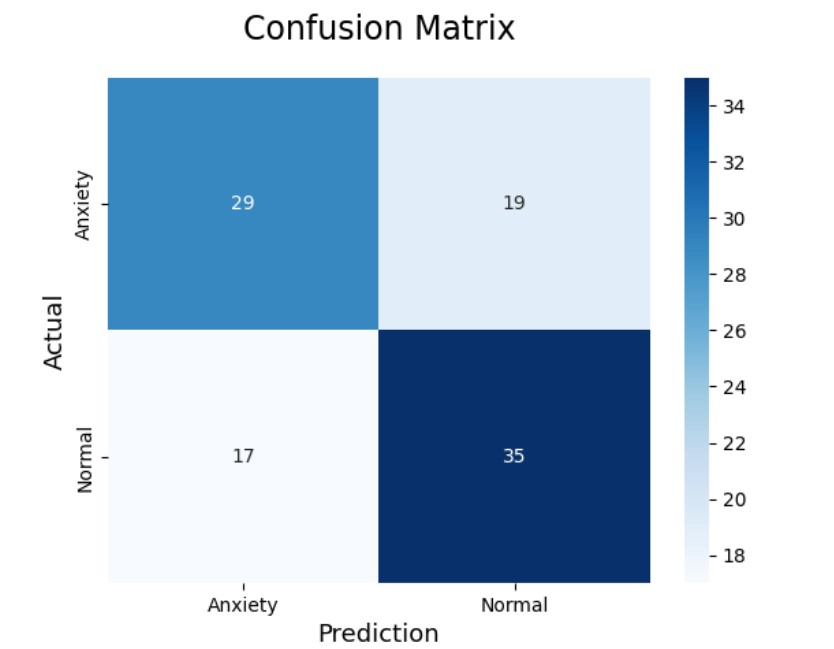
\includegraphics[width=0.9\textwidth]{Anxiety-Data-SmallData.jpg}
\caption[Confusion matrix for anxiety data (small dataset)]{Confusion matrix for anxiety data (small dataset). This matrix shows the classification performance: 29 true positives and 17 false positives for normal cases, and 35 true positives and 19 false negatives for anxiety cases.}
\end{figure}


\vspace{0.5cm} % Add 1 cm of vertical space (adjust as needed)

\subsection{Depression Data}
\label{section:depression}
We used a data set of 500 rows (small data).
\begin{itemize}
    \item \textbf{Hyperparameters:} ID, Text, Target
    \item \textbf{Target:} Normal (249), Depression (251)
    \item \textbf{Models:} Support Vector Classification (Support Vector Machine) with encoding Word2Vec
    \item \textbf{Results:}
    \begin{itemize}
        \item \textbf{Accuracy:} 0.62
        \item \textbf{Precision (average):} 0.6182
        \item \textbf{Precision for Depression Class:} 0.6182
        \item \textbf{Precision for Normal Class:} 0.6222
        \item \textbf{Recall:} 0.6667
        \item \textbf{Confusion Matrix:}
    \end{itemize}
\end{itemize}

\begin{figure}[h]
\centering
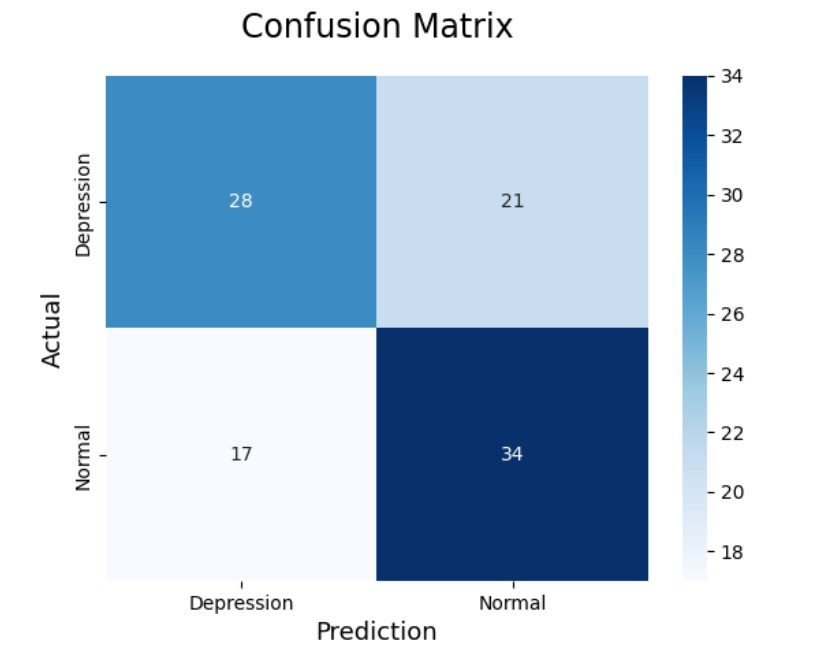
\includegraphics[width=0.9\textwidth]{Depression-Data-SmallData.jpg}
\caption[Confusion matrix for depression data (small dataset)]{Confusion matrix for depression data (small dataset). This matrix illustrates the results with 28 true positives and 17 false positives for normal cases, and 34 true positives and 21 false negatives for depression cases.}
\end{figure}

\vspace{1cm} % Add 1 cm of vertical space (adjust as needed)

\section{Second Approach - Big Data}
\label{section:second}

\subsection{Anxiety Data}
\label{section:anxietydata}

\subsubsection{Linear Regression}
\label{section:linear}

\begin{itemize}
    \item \textbf{Hyperparameters:} ID, Text, Target
    \item \textbf{Target:} Normal (246), Anxiety (254)
    \item \textbf{Models:} Linear Regression with transformer Sentence Transformer with the data set encoding 'all-MiniLM-L6-v2'
    \item \textbf{Results:}
    \begin{itemize}
        \item \textbf{Accuracy:} 0.82
        \item \textbf{Average Precision:} 0.82
        \item \textbf{Precision for Anxiety Class:} 0.82
        \item \textbf{Precision for Normal Class:} 0.82
        \item \textbf{Recall for Anxiety Class:} 0.81
        \item \textbf{Recall for Normal Class:} 0.83
        \item \textbf{Confusion Matrix:}
    \end{itemize}
\end{itemize}

\begin{figure}[h]
\centering
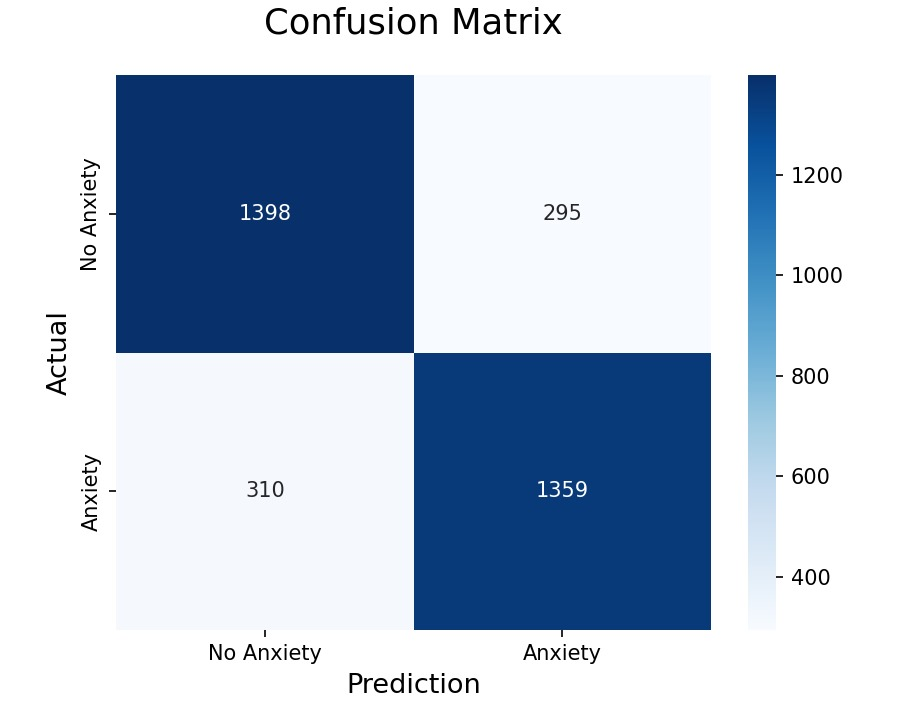
\includegraphics[width=0.9\textwidth]{Anxiety-Data-LinearRegression.jpg}
\caption[Confusion matrix for anxiety data (linear regression)]{Confusion matrix for anxiety data using Linear Regression (large dataset). It details 1398 true positives and 310 false positives for normal cases, along with 1359 true positives and 295 false negatives for anxiety cases.}
\end{figure}

\vspace{1cm} % Add 1 cm of vertical space (adjust as needed)

\subsubsection{Decision Tree}
\label{section:decision}

\begin{itemize}
    \item \textbf{Hyperparameters:} ID, Text, Target
    \item \textbf{Target:} Normal (246), Anxiety (254)
    \item \textbf{Models:} Decision Tree with transformer Sentence Transformer with the data set encoding 'all-MiniLM-L6-v2'
    \item \textbf{Results:}
    \begin{itemize}
        \item \textbf{Accuracy:} 0.83
        \item \textbf{Average Precision:} 0.83
        \item \textbf{Precision for Anxiety Class:} 0.88
        \item \textbf{Precision for Normal Class:} 0.79
        \item \textbf{Recall for Anxiety Class:} 0.75
        \item \textbf{Recall for Normal Class:} 0.90
        \item \textbf{Confusion Matrix:}
    \end{itemize}
\end{itemize}

\begin{figure}[h]
\centering
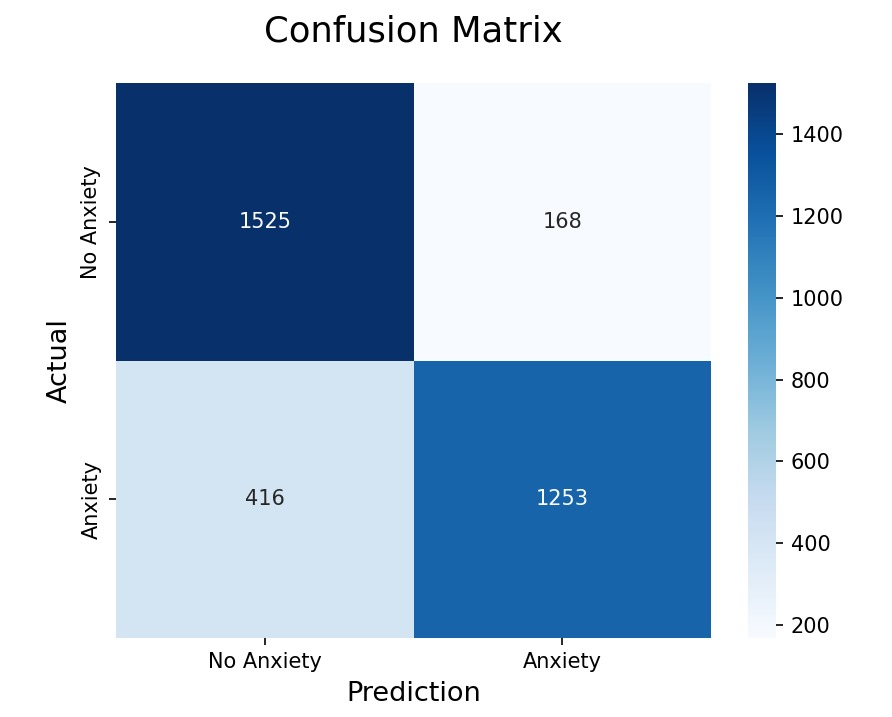
\includegraphics[width=0.9\textwidth]{Anxiety-Data-DecisionTree.jpg}
\caption[Confusion matrix for anxiety data (decision tree)]{Confusion matrix for anxiety data using a Decision Tree (large dataset). The matrix indicates 1525 true positives and 416 false positives for normal cases, with 1253 true positives and 168 false negatives for anxiety cases.}
\end{figure}

\vspace{0.5cm} % Add 1 cm of vertical space (adjust as needed)

\subsubsection{Multi-layer Perceptron Classifier}
\label{section:mpl}

\begin{itemize}
    \item \textbf{Hyperparameters:} ID, Text, Target
    \item \textbf{Target:} Normal (246), Anxiety (254)
    \item \textbf{Models:} Multi-layer Perceptron Classifier with transformer Sentence Transformer with the data set encoding 'all-MiniLM-L6-v2'
    \item \textbf{Results:}
    \begin{itemize}
        \item \textbf{Accuracy:} 0.93
        \item \textbf{Average Precision:} 0.93
        \item \textbf{Precision for Anxiety Class:} 0.95
        \item \textbf{Precision for Normal Class:} 0.90
        \item \textbf{Recall for Anxiety Class:} 0.90
        \item \textbf{Recall for Normal Class:} 0.95
        \item \textbf{Confusion Matrix:}
    \end{itemize}
\end{itemize}

\begin{figure}[h]
\centering
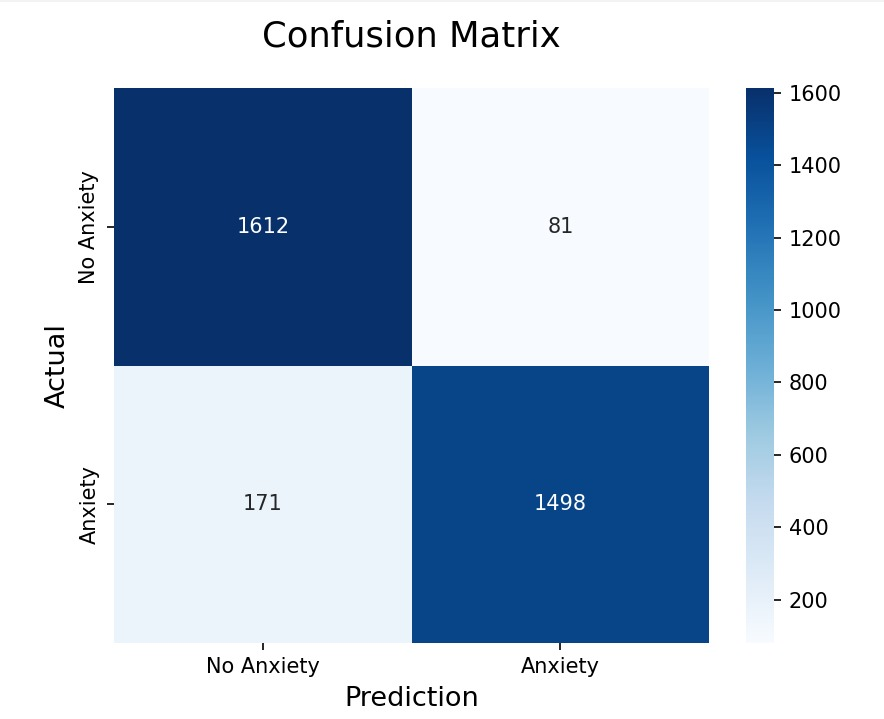
\includegraphics[width=0.9\textwidth]{Anxiety-Data-MLPClassifier.jpg}
\caption[Confusion matrix for anxiety data (Multi-layer Perceptron Classifier)]{Confusion matrix for anxiety data using an Multi-layer Perceptron Classifier (large dataset). It shows 1612 true positives and 171 false positives for normal cases, and 1498 true positives with 81 false negatives for anxiety cases.}
\end{figure}

\vspace{0.5cm} % Add 1 cm of vertical space (adjust as needed)

\subsection{Depression Data}
\label{section:depressiondata}

\subsubsection{Linear Regression}
\label{section:regression}

\begin{itemize}
    \item \textbf{Hyperparameters:} ID, Text, Target
    \item \textbf{Target:} Normal (249), Depression (251)
    \item \textbf{Models:} Linear Regression with transformer Sentence Transformer with the data set encoding 'all-MiniLM-L6-v2'
    \item \textbf{Results:}
    \begin{itemize}
        \item \textbf{Accuracy:} 0.80
        \item \textbf{Average Precision:} 0.81
        \item \textbf{Precision for Depression Class:} 0.81
        \item \textbf{Precision for Normal Class:} 0.80
        \item \textbf{Recall for Depression Class:} 0.80
        \item \textbf{Recall for Normal Class:} 0.81
        \item \textbf{Confusion Matrix:}
    \end{itemize}
\end{itemize}

\begin{figure}[h]
\centering
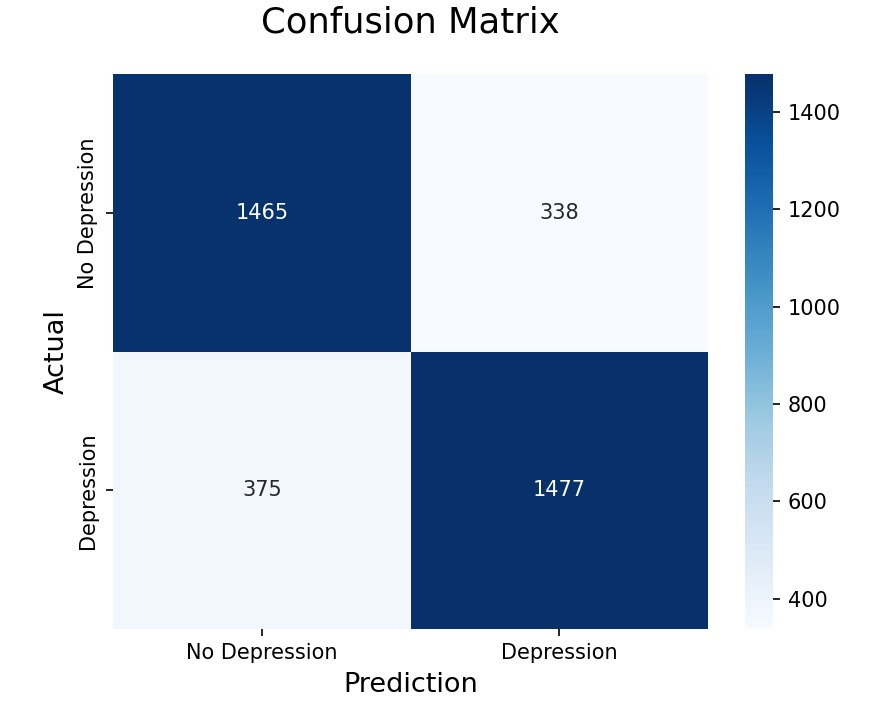
\includegraphics[width=0.9\textwidth]{Depression-Data-LinearRegression.jpg}
\caption[Confusion matrix for depression data (linear regression)]{Confusion matrix for depression data using Linear Regression (large dataset). The results include 1465 true positives and 375 false positives for normal cases, as well as 1477 true positives and 338 false negatives for depression cases.}
\end{figure}

\vspace{0.5cm} % Add 1 cm of vertical space (adjust as needed)

\subsubsection{Decision Tree}
\label{section:tree}

\begin{itemize}
    \item \textbf{Hyperparameters:} ID, Text, Target
    \item \textbf{Target:} Normal (249), Depression (251)
    \item \textbf{Models:} Decision Tree with transformer Sentence Transformer with the data set encoding 'all-MiniLM-L6-v2'
    \item \textbf{Results:}
    \begin{itemize}
        \item \textbf{Accuracy:} 0.83
        \item \textbf{Average Precision:} 0.84
        \item \textbf{Precision for Depression Class:} 0.89
        \item \textbf{Precision for Normal Class:} 0.78
        \item \textbf{Recall for Depression Class:} 0.75
        \item \textbf{Recall for Normal Class:} 0.91
        \item \textbf{Confusion Matrix:}
    \end{itemize}
\end{itemize}

\begin{figure}[h]
\centering
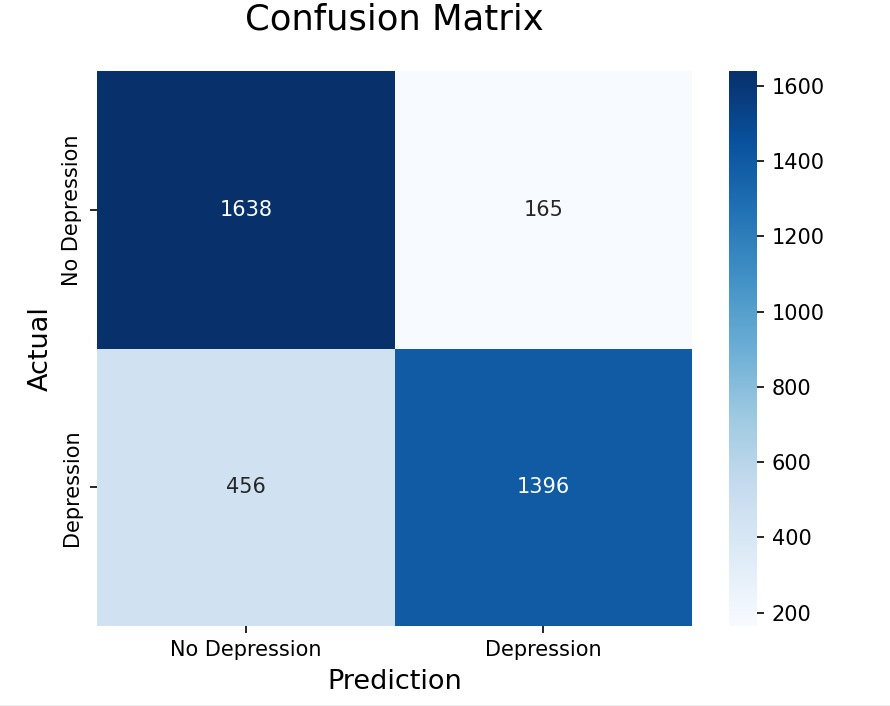
\includegraphics[width=0.9\textwidth]{Depression-Data-DecisionTree.jpg}
\caption[Confusion matrix for depression data (decision tree)]{Confusion matrix for depression data using a Decision Tree (large dataset). It highlights 1638 true positives and 456 false positives for normal cases, with 1396 true positives and 165 false negatives for depression cases.}
\end{figure}

\vspace{0.5cm} % Add 1 cm of vertical space (adjust as needed)

\newpage
\subsubsection{Multi-layer Perceptron Classifier}
\label{section:classifier}
\begin{itemize}
    \item \textbf{Hyperparameters:} ID, Text, Target
    \item \textbf{Target:} Normal (249), Depression (251)
    \item \textbf{Models:} Decision Tree with transformer Sentence Transformer with the data set encoding 'all-MiniLM-L6-v2'
    \item \textbf{Results:}
    \begin{itemize}
        \item \textbf{Accuracy:} 0.93
        \item \textbf{Average Precision:} 0.93
        \item \textbf{Precision for Depression Class:} 0.96
        \item \textbf{Precision for Normal Class:} 0.90
        \item \textbf{Recall for Depression Class:} 0.89
        \item \textbf{Recall for Normal Class:} 0.97
        \item \textbf{Confusion Matrix:}
    \end{itemize}
\end{itemize}

\begin{figure}[h]
\centering
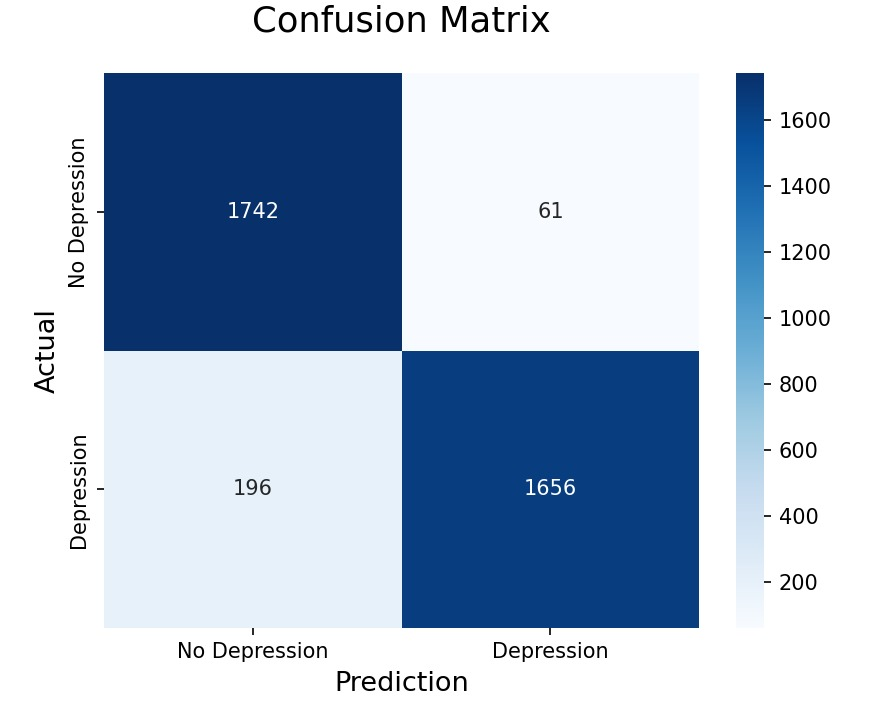
\includegraphics[width=0.9\textwidth]{Depression-Data-MLPClassifier.jpg}
\caption[Confusion matrix for depression data ( Multi-layer Perceptron Classifier)]{Confusion matrix for depression data using an  Multi-layer Perceptron Classifier (large dataset). The matrix reports 1742 true positives and 196 false positives for normal cases, alongside 1656 true positives and 61 false negatives for depression cases.}
\end{figure}

\section{Final Approach}
\label{final-approach}
\subsection{Multi-class Classification Data }
\label{section:multi-class-data}
\subsubsection{Random Forest Classifier}
\begin{itemize}
    \item \textbf{Hyperparameters:} ID, Text, Target
    \item \textbf{Target:} Normal (16543), Anxiety(16576), Depression (16456)
    \item \textbf{Models:} Random Forest Classifier with the data set encoding TF-IDF Vectorizer
    \item \textbf{Results:}
    \begin{itemize}
        \item \textbf{Accuracy:} 0.92 
        \item \textbf{Cross-Validation Accuracy:} 0.9202
        \item \textbf{Average Precision:} 0.92
        \item \textbf{Precision for Anxiety Class:} 0.95
        \item \textbf{Precision for Depression Class:} 0.88
        \item \textbf{Precision for Normal Class:} 0.95
        \item \textbf{Recall for Anxiety Class:} 0.91
        \item \textbf{Recall for Depression Class:} 0.91
        \item \textbf{Recall for Normal Class:} 0.93
        \item \textbf{Confusion Matrix:}
    \end{itemize}
\end{itemize}

\begin{figure}[H]
\centering
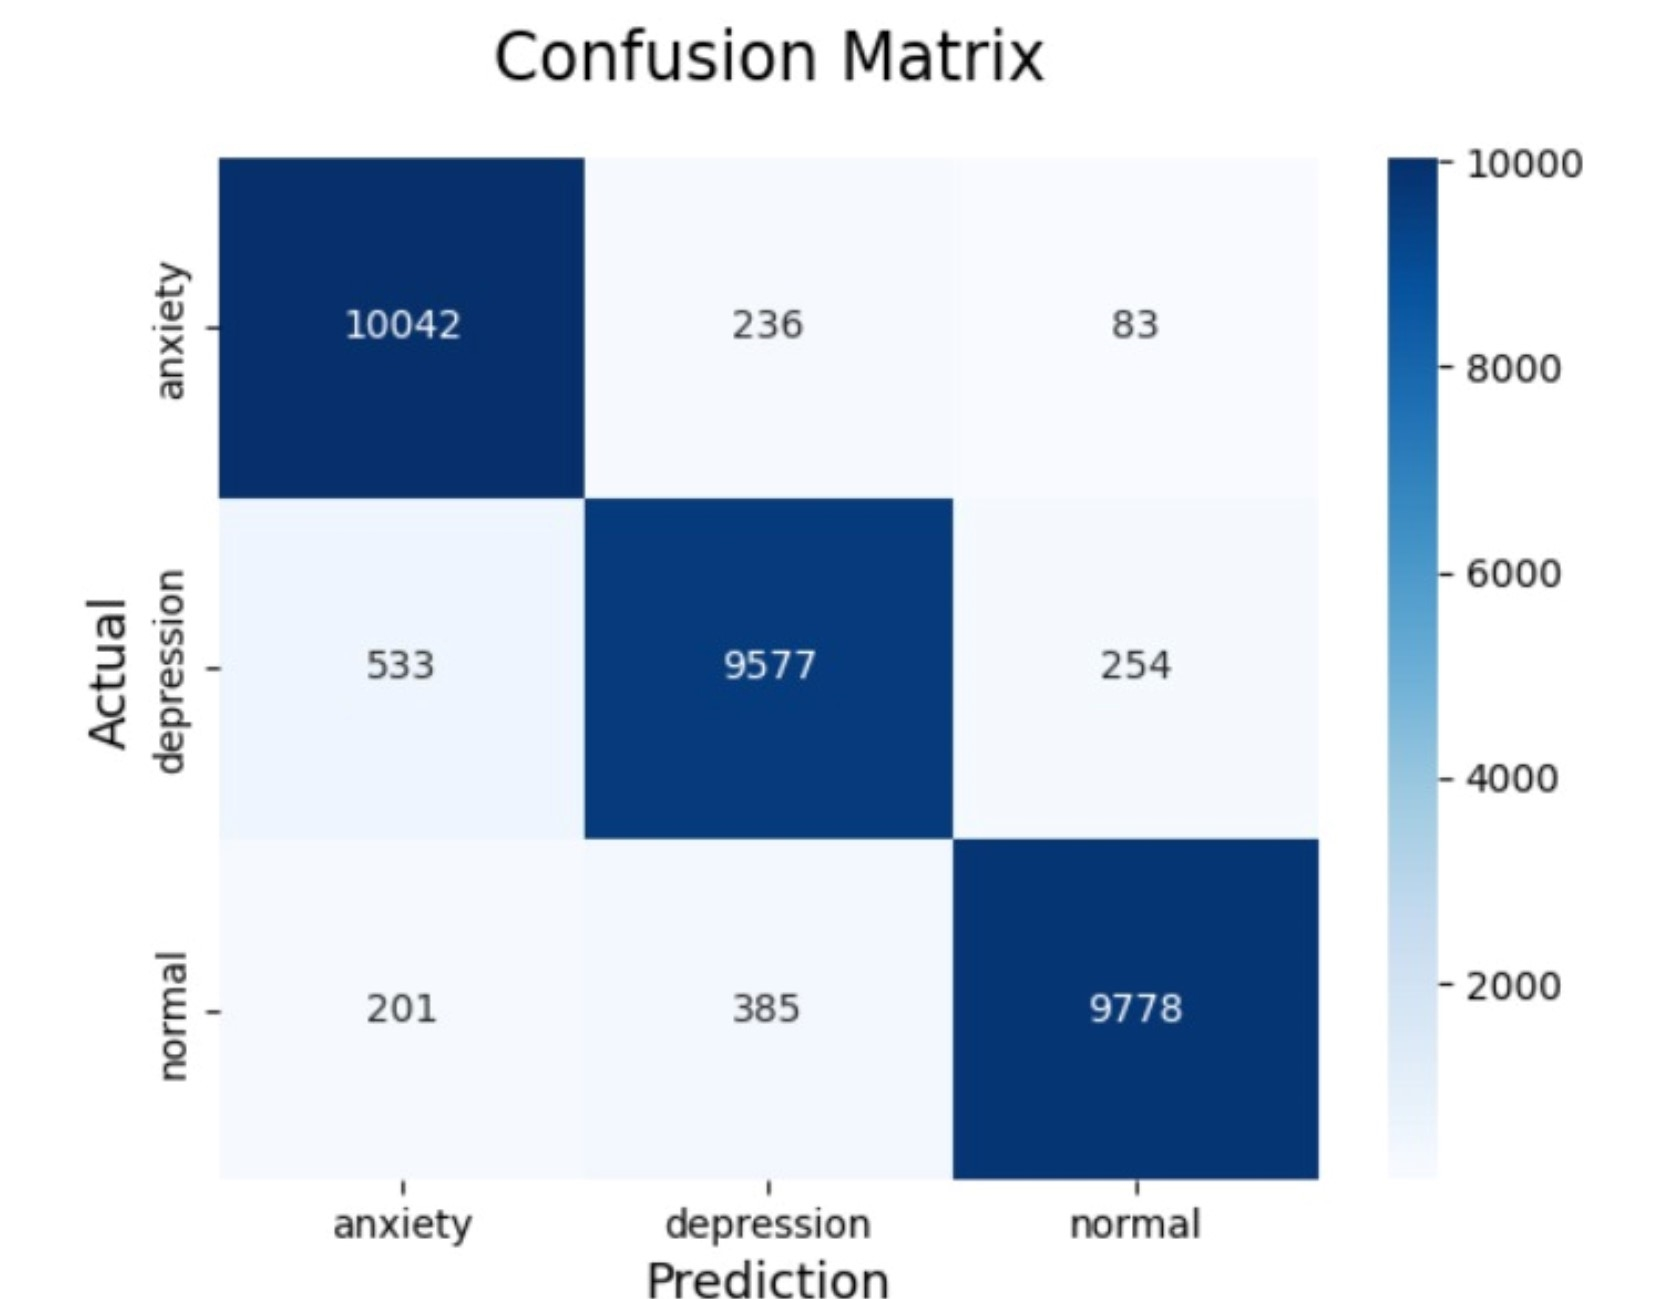
\includegraphics[width=0.8\textwidth]{Multi-Class-Data.jpg}
\caption[Confusion matrix for mental health classification (Random Forest Classifier)]{Confusion matrix for mental health classification using a Random Forest Classifier. The matrix indicates the model's performance with 10042 true positives and 734 misclassifications for anxiety, 9577 true positives and 621 misclassifications for depression, and 9778 true positives with 337 misclassifications for normal cases.}
\label{fig:confusion_matrix_rf}
\end{figure}
\clearpage


\section{Spatial Complexity}
\label{section:spatial-complexity}

\subsection{What It Means}
\label{section:what-it-means}
Spatial complexity refers to the memory required during the execution of the code. It depends on the size of data structures stored in memory, including intermediate and final outputs.

\subsection{Code Analysis}
\label{section:code}

\subsubsection{TF-IDF Vectorizer}
\label{section:tf-idf}
\begin{itemize}
  \item \textbf{Details:} Converts text into a sparse matrix of size $n \times m$, where:
  \begin{itemize}
    \item $n$: Number of documents in the dataset.
    \item $m$: Maximum features defined (\texttt{max\_features=5000} in your case).
  \end{itemize}
  \item \textbf{Spatial Complexity:}
  \[
  O(n \cdot m)
  \]
  The memory usage grows linearly with the number of documents and features. For sparse data (most elements being zero), storage efficiency improves.
\end{itemize}

\subsubsection{Random Forest Classifier}
\label{section:random-classifier}
\begin{itemize}
  \item \textbf{Details:} The Random Forest classifier uses $t$ trees, each with nodes storing:
  \begin{itemize}
    \item Splitting features,
    \item Threshold values,
    \item Branches for splits until maximum tree depth ($d$).
  \end{itemize}
  \item \textbf{Spatial Complexity:}
  \[
  O(t \cdot d \cdot f)
  \]
  Here, $t$ is the number of trees, $d$ is the depth of each tree, and $f$ is the features used per split. As $t$ or $d$ increases, memory usage scales proportionally.
\end{itemize}

\subsubsection{Dataset Storage}
\label{section:data-storage}
\begin{itemize}
  \item \textbf{Details:} The dataset is stored in a \texttt{pandas DataFrame} and requires memory for:
  \begin{itemize}
    \item Raw text ($n \cdot \text{average text length}$),
    \item Labels ($n$),
    \item Vectorized text ($n \cdot m$).
  \end{itemize}
  \item \textbf{Spatial Complexity:}
  \[
  O(n \cdot m + n)
  \]
  The majority of memory is consumed by the vectorized text.
\end{itemize}

\subsubsection{Model Serialization}
\label{section:model}
\begin{itemize}
  \item \textbf{Details:} The model is saved using \texttt{joblib}, which includes:
  \begin{itemize}
    \item The Random Forest classifier (including trees, features, and splits),
    \item The TfidfVectorizer (vocabulary and IDF values).
  \end{itemize}
  \item \textbf{Spatial Complexity:}
  \[
  O(t \cdot d \cdot f + m)
  \]
  This scales with the complexity of the classifier and vectorizer.
\end{itemize}

\subsubsection{Confusion Matrix}
\label{section:confusion}
\begin{itemize}
  \item \textbf{Details:} The confusion matrix is stored as a $c \times c$ grid, where $c$ is the number of classes.
  \item \textbf{Spatial Complexity:}
  \[
  O(c^2)
  \]
  Memory requirements here are negligible compared to other components.
\end{itemize}

\subsection{Overall Spatial Complexity}
\label{section:overall-spatial}
Combining all components:
\[
O(n \cdot m + t \cdot d \cdot f + c^2)
\]
Where:
\begin{itemize}
  \item $n$: Number of documents,
  \item $m$: Features in the vectorizer (5000 in this case),
  \item $t$: Trees in the Random Forest (200),
  \item $d$: Depth of each tree,
  \item $f$: Features considered per split,
  \item $c$: Number of classes.
\end{itemize}

\subsection{Example Impact}
\label{section:example-spatial}
For a dataset with:
\begin{itemize}
  \item $n = 10,000$ (documents),
  \item $m = 5000$ (features),
  \item $t = 200$ (trees),
  \item $d = 10$ (depth),
  \item $f = 50$ (features per split),
  \item $c = 3$ (classes):
\end{itemize}

\begin{enumerate}
  \item \textbf{Vectorized Data:} $10,000 \cdot 5000 = 50,000,000$ elements (approx. 190 MB in sparse format).
  \item \textbf{Random Forest:} $200 \cdot 10 \cdot 50 = 100,000$ elements per tree, totaling $20,000,000$ elements (approx. 76 MB).
  \item \textbf{Confusion Matrix:} $3^2 = 9$ elements (negligible).
\end{enumerate}

\textbf{Total Memory Impact:} Around 266 MB for processing and storing the model.

Increasing $t$ (trees) or $d$ (depth) will significantly increase memory usage, making scalability an important factor to consider.

\newpage
\section{Temporal Complexity}

\subsection{What It Means}
\label{section:it-means}
Temporal complexity refers to the runtime or the computational cost of executing the program, expressed in terms of how operations grow with input size.

\subsection{Code Analysis}
\label{section:codeAnalysis}

\subsubsection{TF-IDF Vectorizer}
\label{section:vectorizer}
\begin{itemize}
  \item \textbf{What happens:}
  \begin{itemize}
    \item The \texttt{TF-IDF Vectorizer} transforms text data into a numeric representation (a sparse matrix) by:
    \begin{enumerate}
      \item Tokenizing the text into individual words.
      \item Computing term frequencies (TF) for each word in each document.
      \item Calculating the inverse document frequency (IDF) for each word across all documents.
      \item Combining TF and IDF values to create the final matrix.
    \end{enumerate}
  \end{itemize}
  \item \textbf{Temporal Complexity:}
  \[
  O(n \cdot \text{avg\_len} + n \cdot m)
  \]
  The first term accounts for tokenization, and the second term covers matrix computations.
\end{itemize}

\subsubsection{Random Forest Classifier}
\label{section:forest-classifier}
\begin{itemize}
  \item \textbf{What happens:}
  \begin{itemize}
    \item The Random Forest classifier trains $t$ decision trees by:
    \begin{enumerate}
      \item Sampling data with replacement (Bootstrap sampling) from the training set.
      \item Iteratively splitting nodes based on $f$ features (randomly selected) until a stopping condition is met (e.g., tree depth $d$).
      \item Predicting outcomes by aggregating the results from all trees.
    \end{enumerate}
  \end{itemize}
  \item \textbf{Temporal Complexity:}
  \[
  O(t \cdot n \cdot d \cdot f)
  \]
  Prediction involves evaluating all $t$ trees for each document, with complexity:
  \[
  O(t \cdot n)
  \]
\end{itemize}

\subsubsection{Cross-Validation}
\label{section:cross-validation}
\begin{itemize}
  \item \textbf{What happens:}
  \begin{itemize}
    \item Cross-validation splits the training set into $k$ folds and trains the model $k$ times, using $k-1$ folds for training and 1 fold for testing.
  \end{itemize}
  \item \textbf{Temporal Complexity:}
  \[
  O(k \cdot t \cdot n \cdot d \cdot f)
  \]
\end{itemize}

\subsection{Overall Temporal Complexity}
\label{section:overall-temporal}
Summing up:
\[
O(n \cdot \text{avg\_len} + n \cdot m + k \cdot t \cdot n \cdot d \cdot f)
\]


\section{Portability Analysis}
\label{section:portability-analysis}

\subsection{What It Means}
Probability is a measure quantifying the likelihood that an event will occur. It is expressed as a number between 0 and 1, where 0 indicates impossibility and 1 indicates certainty. Mathematically, the probability \( P(E) \) of an event \( E \) is defined as:
\[
P(E) = \frac{\text{Number of favorable outcomes}}{\text{Total number of possible outcomes}}
\]
Probability is a fundamental concept in statistics and machine learning, often used to predict outcomes and assess model confidence.

\subsection{Code Analysis}
\label{section:code_analysis}

\subsubsection{File Path Handling}
\label{section:file-path-handaling}
\textbf{Current Situation:} The code uses hardcoded, absolute paths such as:
\begin{verbatim}
data = pd.read_csv(
    "../data/anxiety_depression_data.csv"
)

joblib.dump(
    model, 
    "../multiclass_classifiers/model_3_class_classifier_random_forests.joblib"
)
\end{verbatim}
These paths make the code dependent on a specific directory structure, which is not portable across systems.

\textbf{Solution:} Replace absolute paths with relative paths or configurable paths using the \texttt{os} module:
\begin{verbatim}
import os

data_path = os.path.join(
    "app", 
    "data", 
    "anxiety_depression_data.csv"
)
data = pd.read_csv(data_path)

model_path = os.path.join(
    "app", 
    "persistency", 
    "model_3_class_classifier_random_forests.joblib"
)
joblib.dump(model, model_path)
\end{verbatim}

\subsubsection{Library Dependencies}
\label{section:library-dependencies}
\textbf{Current Situation:} The code does not specify exact versions of dependencies, leading to inconsistencies across environments.

\textbf{Solution:} Create a \texttt{requirements.txt} file to pin the library versions. Example:
\begin{verbatim}
pandas==1.5.3
scikit-learn==1.2.0
matplotlib==3.6.2
seaborn==0.12.2
joblib==1.2.0
\end{verbatim}
Use \texttt{pip install -r requirements.txt} to set up dependencies.

\subsubsection{Operating System Compatibility}
\label{section:os-comatibility}
\textbf{Current Situation:} The code uses Windows-style paths (\texttt{C:/...}), which are incompatible with Linux/macOS.

\textbf{Solution:} Use platform-agnostic paths via the \texttt{os} module:
\begin{verbatim}
os.path.join(
    "directory", 
    "file.csv"
)
\end{verbatim}

\subsubsection{Deployment Across Languages/Platforms}
\label{section:deployment-across}
\textbf{Optional Improvement:} If the model needs to be deployed in non-Python environments, consider exporting it to a universal format like ONNX:
\begin{verbatim}
from skl2onnx import convert_sklearn

onnx_model = convert_sklearn(
    model, 
    initial_types=[('input', FloatTensorType([None, 5000]))]
)
\end{verbatim}

\subsubsection{Environment Configuration}
\label{section:enviroment-configuration}
\textbf{Current Situation:} Environment variables like file paths or runtime configurations are hardcoded.

\textbf{Solution:} Use environment variables or configuration files to store such settings.

\subsection{Summary}
\label{section:summary}
To make the code portable:
\begin{enumerate}
    \item Replace absolute file paths with relative ones.
    \item Use a \texttt{requirements.txt} file for dependency management.
    \item Avoid OS-specific code and use platform-agnostic methods for file handling.
    \item \textit{(Optional)} Export the model to a cross-platform format for deployment in non-Python environments.
    \item Use environment variables or configuration files for runtime settings.
\end{enumerate}

\chapter{Conclusions and Possible Improvements}
\label{chapter:conclusions}

\section{Conclusions}
The study presents an innovative approach to addressing the growing prevalence of anxiety and depression among teenagers by leveraging digital platforms and advanced AI technologies. By focusing on early detection and personalized intervention, the proposed system offers a scalable and proactive solution that meets teenagers where they naturally engage — in their digital environments.

The implementation of algorithms such as Support Vector Machines (SVM), Random Forest Classifiers, Decision Trees, and Transformer-based Neural Networks showcases the potential of combining traditional machine learning techniques with state-of-the-art AI tools for natural language processing. The integration of datasets such as the \textit{Reddit Mental Health Dataset} and \textit{Emotion Recognition Dataset} provided a rich source of diverse features, enabling the models to learn complex emotional patterns.

Key conclusions drawn from the study include:

\begin{itemize}
    \item \textbf{Effectiveness of AI in Mental Health Classification:} Models leveraging sentence embeddings and TF-IDF vectors demonstrated strong performance in categorizing emotional states as anxiety, depression, or normal. This highlights the potential of AI to identify subtle cues in textual data indicative of mental health challenges.
    \item \textbf{Importance of Data Balance:} Oversampling and careful data preprocessing significantly improved model accuracy and reduced biases, ensuring that each class (Anxiety, Depression, and Normal) was equally represented during training.
    \item \textbf{Transformer Models' Superior Performance:} Neural network architectures utilizing transformers like \textit{all-MiniLM-L6-v2} provided the most robust results in capturing semantic context and subtle nuances in text. This reaffirms the utility of advanced embeddings for tasks involving unstructured data.
\end{itemize}

\section{Limitations}
Despite the promising results, the study faced several limitations that warrant further exploration:

\begin{itemize}
    \item \textbf{Computational Complexity:} Transformer-based models, while powerful, required significant computational resources for training and inference. This limits their deployability in low-resource environments.
    \item \textbf{Dataset Generalizability:} While the combined dataset was balanced and diverse, it may not capture cultural or linguistic variations in how mental health issues are expressed.
    \item \textbf{Lack of Real-Time Validation:} The study relied on static datasets, and the models have not yet been tested in real-world scenarios where real-time interactions may introduce additional challenges.
    \item \textbf{Sensitivity to Ambiguity:} Models occasionally struggled with ambiguous or mixed emotional signals, highlighting the need for more advanced techniques to handle complex, multi-faceted emotional states.
\end{itemize}

\section{Possible Improvements} 
To further enhance the proposed system and address its limitations, the following improvements are recommended:

\begin{itemize} 
    \item \textbf{Incorporation of Multimodal Data:} Future work could integrate additional data sources, such as voice tone analysis, facial expressions, and physiological data, to provide a more comprehensive view of a teenager's mental state. 
    \item \textbf{Continuous Learning:} Implementing mechanisms for models to learn and adapt over time using real-world feedback will ensure their relevance in evolving digital environments. 
    \item \textbf{Diversification of Data Sources:} Expanding the dataset with examples from varied sources, such as forums, blogs, and different social media platforms, would enrich the training data and improve the model’s robustness across diverse contexts. 
    \item \textbf{Real-Time Data Collection:} Implementing automated mechanisms for the continuous extraction of updated data from online sources would allow the system to remain relevant and up-to-date with current trends and behaviors. 
    \item \textbf{Adaptation to Regional Specifics:} Integrating data from different languages and cultures to reflect linguistic and socio-cultural diversity would ensure that the system is effective across various global contexts and user demographics.

\end{itemize}

\section{Final Remarks}
This project underscores the transformative potential of AI-driven tools in addressing teenage mental health challenges. By identifying and addressing key limitations, future iterations of the system can further refine its accuracy, accessibility, and effectiveness. Through collaborative efforts between technologists, mental health professionals, and educators, this solution can make significant strides toward reducing the stigma of mental health and providing timely support to those in need.


\newpage
\addcontentsline{toc}{chapter}{Bibliography} 
\begin{thebibliography}{99}

\bibitem{depression_reddit_cleaned}  
\textit{Depression Reddit Dataset (Cleaned)}.  
Infamous Coder (2020).  
\\Available at: \url{https://www.kaggle.com/datasets/infamouscoder/depression-reddit-cleaned}.  

\bibitem{emotion_dataset}  
\textit{Emotion Dataset}.  
Parul Pandey (2020).  
\\Available at: \url{https://www.kaggle.com/datasets/parulpandey/emotion-dataset/data?select=training.csv}.  

\bibitem{emotions}  
\textit{Emotions Dataset}.  
Nelgiriyewithana (2020).  
\\Available at: \url{https://www.kaggle.com/datasets/nelgiriyewithana/emotions}.  

\bibitem{reddit_dataset} 
\textit{Reddit Mental Health Dataset}.  
Neel Ghoshal (2020).  
\\Available at: \url{https://www.kaggle.com/datasets/neelghoshal/reddit-mental-health-data}. 

\bibitem{students_anxiety_depression}  
\textit{Students Anxiety and Depression Dataset}.  
Saha Sourav (2020).  
\\Available at: \url{https://www.kaggle.com/datasets/sahasourav17/students-anxiety-and-depression-dataset}.  

\end{thebibliography}




\end{document}